\section{Ergebnis} % (fold)
\label{sec:ergebnis}
	Bereits zu Beginn des Projekts war es wichtig es messbar zu machen. Dafür wurde eine Testumgebung aufgebaut, mit deren Hilfe die Seite nach ihrer Geschwindigkeit getestet werden kann. Ganz entscheidend war dabei die Webpagetest API in Verbindung mit Google Spreadsheets. Damit lassen sich regelmäßig automatisierte Tests durchführen und die Daten werden nach erfolgreichem Test automatisch in einer Spreadsheet Tabelle gespeichert. Die über den Zeitraum der Arbeit hinweig gesammelten Daten sind hier finden: \url{http://tinyurl.com/l5usz79}. Diese Daten wurden anschließend mittels \url{http://Chartjs.org} in Diagrammen aufbereitet und alle Diagramme sind auch Online abrufbar unter: \url{http://bithugger.github.io/bachelorthesis/}

	\subsection{Wie wurde getestet?} % (fold)
	\label{sub:wie_wurde_getestet}
		Damit mittels Google Spreadsheets die Webpagetest API verwendet werden kann, ist es nötig einen sogenannten API-Key anzufordern. Ein solcher Key ist kostenlos unter der Adresse: \url{http://www.webpagetest.org/getkey.php} zu erhalten und bietet die Möglichkeit täglich 200 Seitenaufrufe zu tätigen. Als Seitenaufruf zählt sowohl die "`first view"' als auch "`repeat view"'. Die Tests sind 30 Tage abrufbar und gespeichert.\\

		Für das Testen der Seite kann aus einer Vielzahl an Teststandorten gewählt werden. Damit lässt sich nachvollziehen wie beispielsweise die Ladezeiten aus der USA oder Asien sind. Je nach Zielgruppe sollten Tests von verschiedenen Standorten in betracht gezogen werden.\footnote{Eine volle Liste der zur Verfügung stehenden Teststandorte ist im Anhang unter Punkt: \ref{sub:webpagetest_teststandorte} zu finden.} Für dieses Projekt wurden ausschließlich Teststandorte aus der USA und Europa gewählt.\\

		Als Testparameter wurde eine Anzahl von 9 Tests pro Testlauf gewählt. Dabei wurde sowohl die "`first view"' als auch die "`repeat view"' aufgezeichnet. Von den 9 Testläufen wurde der Median als Ergebnis des Testlaufs verwendet. Über den Zeitraum der Arbeit wurde die Seite 1089 Tests unterzogen.\\

		Das größte Problem bestand in der möglichst genauen Messzeiterfassung für die Ladezeiten mittels Smartphone. Webpagetest stellt nur einen Smartphones Teststandort in Dulles USA zu Verfügung. Da die Latenz zwischen dem Hosting in Deutschland und dem Seitenaufruf in der USA sehr viel größer ist, als wenn dieser direkt aus Deutschland erfolgt, wurde nach einer Lösung gesucht diese Messungen exakter zu gestalten.
		Die Lösung dafür ist, ein zweites Hosting mit der selben Seite in den USA zu erstellen. Dafür wurde die "`Microsoft Azure Cloud"' verwendet. Eine kostenlose Testversion ermöglicht es, ganz einfach auf verschiedensten Kontinenten eine Webseite zu hosten. Die Seite wurde für die Tests Online geschaltet und nach den Testläufen wieder Offline genommen.

	% subsection wie_wurde_getestet (end)

	\subsection{Datenauswertung}
	\label{sub:datenauswertung}
		Folgende Daten wurden bei jedem Testlauf erfasst: Speed Index, TTFB (ms), Render start (ms), Visually complete (ms), Dom Content loaded (ms), Site fully loaded (ms), Requests, Bytes in Document.

    Das Diagramm in Abbildung \ref{fig:data_all}, zeigt eine Übersicht der verschiedenen Messwerte über den Zeitraum des Projekts. Die Y-Achse bildet die Zeit in Millisekunden ab und die X-Achse ist das Datum der Messung. Innerhalb von 36 Tagen haben sich alle Werte signifikant verbessert.
    % todo: wirklich 36 Tage? Nachzählen!

    \begin{figure}[htbp]
    	\begin{center}
    		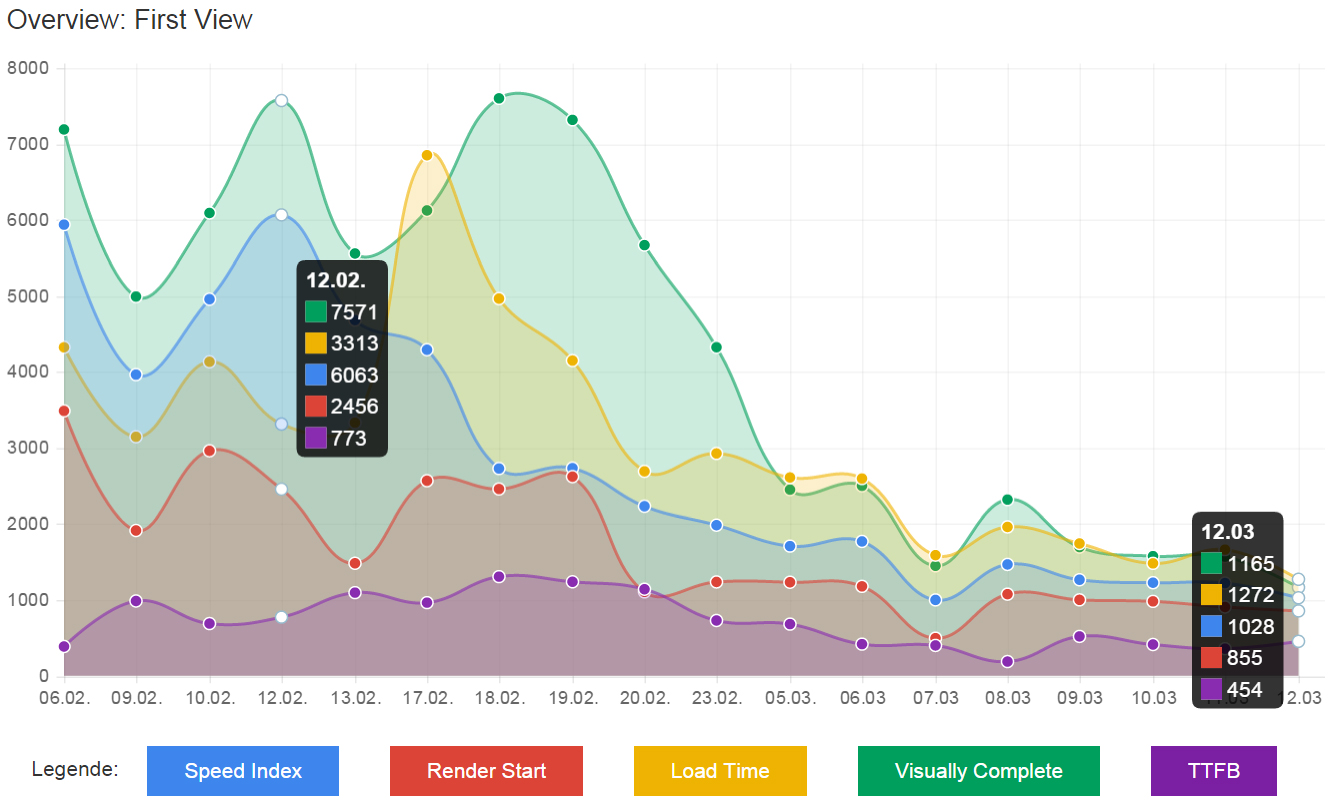
\includegraphics[width=\textwidth]{data_all.jpg}
    		\caption{Datenauswertung - Überblick}
    		\label{fig:data_all}
    	\end{center}
    \end{figure}

    \begin{itemize}
        \item Speed Index: Ein Speed Index von < 1000 Punkten wird als "`schnell genug"' angesehen. Der Median des Speed Indexes konnte von 6063 Zählern auf 1028 Zähler verringert werden. 
        % todo, evt Zitat von Twittter (how fast is fast enough?)
        % fazit: was bedeutet der Speed Index jetzt konkret für den Anwender / Nutzer / fürs Projekt?
        % todo, evt vergleich mit speed index der top 1000 Alexa sites
        \item Render Start: Während dieser Wert bereits bei Projektbeginn mit 2,4 Sekunden für das erste Rendern recht gut war, konnte auch hier fast das dreifache der Zeit (287\%) eingespart werden. Dieser Wert wird durch dieses Diagramm nicht drastisch genug ausgedrückt. So konnte die alte Version der Seite auf dem Smartphone durchaus einen \texttt{Render start} von ganzen 10 Sekunden haben. Das dieser Wert im Diagramm vergleichbar gering ausfällt liegt daran, dass auch viele Tests mittels Desktop PC und Kabelverbindung eingeflossen sind. Die jetzige Renderzeit auf dem Smartphone beträgt ungefähr 1,4 Sekunden. 
        % note: daten, die den render start von 1,4 sec belegen?
        \item Load Time bestimmt, wie lange ein Anwender warten muss, bis eine Interaktion mit der Seite möglich ist. Dieser Wert konnte um volle 2 Sekunden verringert werden. Dies wurde vor allem durch eine verringerung der Seitengröße erreicht.
        % nachprüfen ob das mit der Interaktionszeit so stimmt
        \item Visually Complete: Der höchste Messwert mit rund 7,6 Sekunden konnte auf 1,2 Sekunden verringert werden. Der Hauptgrund dafür ist die Priorisierung des Inhalts "`above the fold"'. Bei der alten Version erfolgte keine priorisierung, welche Bilder zuerst und welche zuletzt geladen werden sollen. Dadurch konnte es sein, dass Bilder die sehr weit unten platziert waren, zuerst geladen wurden was die "`Visually Complete"' Zeit erhöhte. In der neuen Version wird alles, was unterhalb des "`above the fold"' ist verzögert geladen.
        \item TTFB: Dieser Wert ist grundsätzlich nicht beeinflussbar und sollte durch die Wahl des richtigen Hosting Anbieters so niedrig wie möglich gehalten werden.
    \end{itemize}
    \pagebreak

		\begin{figure}[htbp]
			\begin{center}
				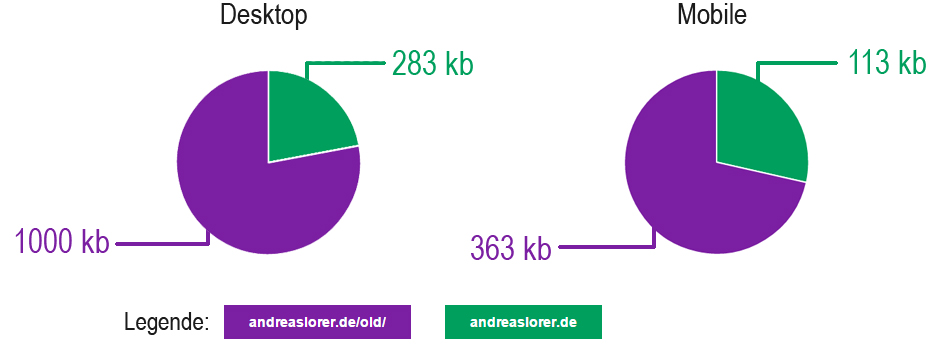
\includegraphics[width=0.8\textwidth]{site_size_in_kb.jpg}
				\caption{Seitengröße in Kilobyte}
				\label{fig:site_size_in_kb}
			\end{center}
		\end{figure}

		Die Seitengröße konnte in der Mobilen und Desktop Variante um rund 3/4 reduziert werden. Dadurch sinkt für den Anwender nicht nur die Ladezeit, sondern auch sein Datenvolumen wird weniger in Anspruch genommen. Laut \url{http://whatdoesmysitecost.com/site/andreaslorer.de} kostet ein Seitenaufruf zwischen 0,01\$ und 0,04\$. Die reduzierung wurde durch mehrere Dinge erreicht: 
		\begin{itemize}
			\item Die "`best practices"' wurden umgesetzt und der Server, wie oben beschrieben, entsprechend konfiguriert.
			\item Bilder "`below the fold"' werden erst dann geladen, wenn der Anwender dort hin scrollt.
			\item Bilder wurden umfassend Komprimiert und \texttt{Progressive} abgespeichert
			\item Das Framework wurde von Bootstrap auf \texttt{Pure.css} gewechselt.
			\item Verwendung von "`Responsive Images"'.
			\item Es werden mittels \texttt{Fontello} nur die Icons geladen, die auch in der Seite eine Verwendung finden.
			\item JQuery wurde als Abhängigkeit für die Bildergallery entfernt. Dadurch kann das herunterladen von JQuery soweit verzögert werden, bis alle wichtigen Teile der Seite geladen wurden. 
			\begin{figure}[htbp]
				\begin{center}
					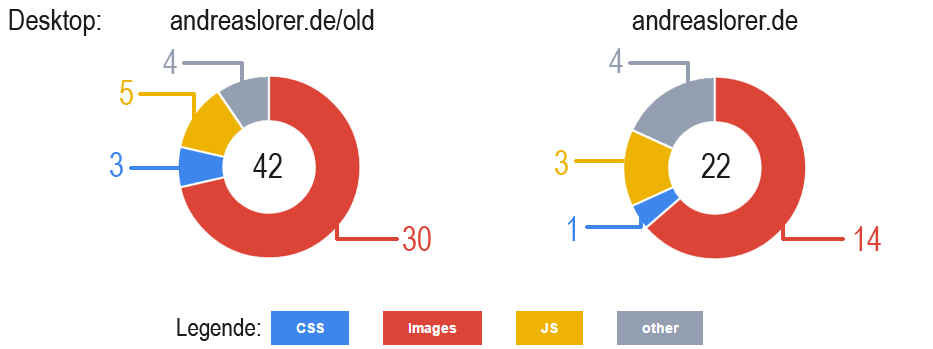
\includegraphics[width=0.8\textwidth]{amount_of_requests.jpg}
					\caption{Anzahl an Requests via Desktop}
					\label{fig:amount_of_requests}
				\end{center}
			\end{figure}
			\item Scripts und sonstige Ressourcen wurden verkleinert und zusammengefasst. Die Anzahl an Requests wurde in der Desktop Variante um die Hälfte verringert.

			\begin{figure}[htbp]
				\begin{center}
					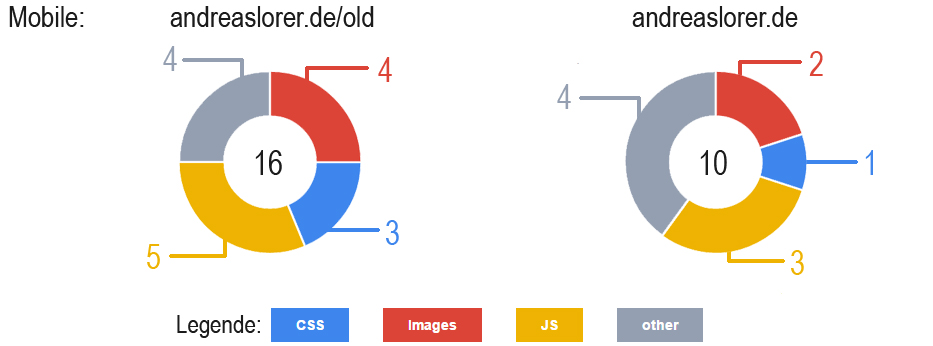
\includegraphics[width=0.8\textwidth]{amount_of_requests_mobile.jpg}
					\caption{Anzahl an Requests via Mobile}
					\label{fig:amount_of_requests_mobile}
				\end{center}
	    \end{figure}

			\item In der Mobilen Variante konnten weitere Requests eingespart werden und es wird nur noch der Hintergrund und das erste Bild der Bildergallery geladen.
		\end{itemize}

		Beim Seitenaufruf mittels Desktop-PC und Kabelverbindung können "`first Render"' Zeiten von unter 189 ms und ein Speed Index von 468 erreicht werden.\footnote{Test Desktop: \url{http://www.webpagetest.org/result/150324_EW_105M/5/details/}} Auf Smartphones mit 3G Netz und 300 ms RTT siehen die Werte etwas schlechter aus und so kann je nach Tag oder Uhrzeit das Ergebnis entsprechend anders ausfallen. Hier sind Werte von 1,3 Sekunden bis zum "`first Render"' und einem Speed Index von 1948 möglich.\footnote{Test Mobile: \url{http://www.webpagetest.org/result/150308_5V_JSD/4/details/}}. Ein visueller Vergleich zwischen der alten und neuen Seite ist in Form eines Videos unter der URL: \url{http://tinyurl.com/o8xoy7m} zu sehen.
		

	% subsection datenauswertung (end)
% section ergebnis (end)



\pagebreak




\section{Der Weg zur Performance} % (fold)
\label{sec:der_weg_zur_performance}
	Damit Webanwendungen überhaupt eine gute Performance  bieten können, gibt es eine fundamentale Bedingung: Sowohl das ganze Team als auch das ganze Unternehmen muss hinter dem Gedanken "`Speed is feature number one"'\autocite{holzle10} stehen. Diese Voraussetzung zu erfüllen und alle in ein "`Boot"' zu bekommen kann bereits sehr schwierig sein, ist aber für den Erfolg einer schnellen Webanwendung unabdingbar.

	\begin{quote}
		\textit{"`Performance more often comes down to a cultural challenge, rather than simply a technical one."'} \autocite[p. 13]{kovalcin15}

		\textit{"`If other designers and developers who shape the site aren’t educated on performance, how can they make the best decisions about user experience? How can they weigh the balance between aesthetics and page speed? If they aren’t empowered to make improvements, any performance champions will simply be playing cleanup after other people’s work. Spending your time cleaning up other people’s work (especially when it’s preventable) is a one-way ticket to burnout."'} \autocite{hogan14}
	\end{quote}

	Damit dies gelingt beschäftigt sich dieser Abschnitt mit der Frage, wie der Weg zur Web Performance aussehen kann und welche Hürden es zu meistern gibt.

	\subsection{Hürden} % (fold)
	\label{sub:hürden}
	
	Wenn man an das Thema Web Performance denkt, so mag man in erster Linie denken, dass dies ausschließlich für die Developer von Belangen ist.
	
	\begin{figure}[htbp]
		\begin{center}
			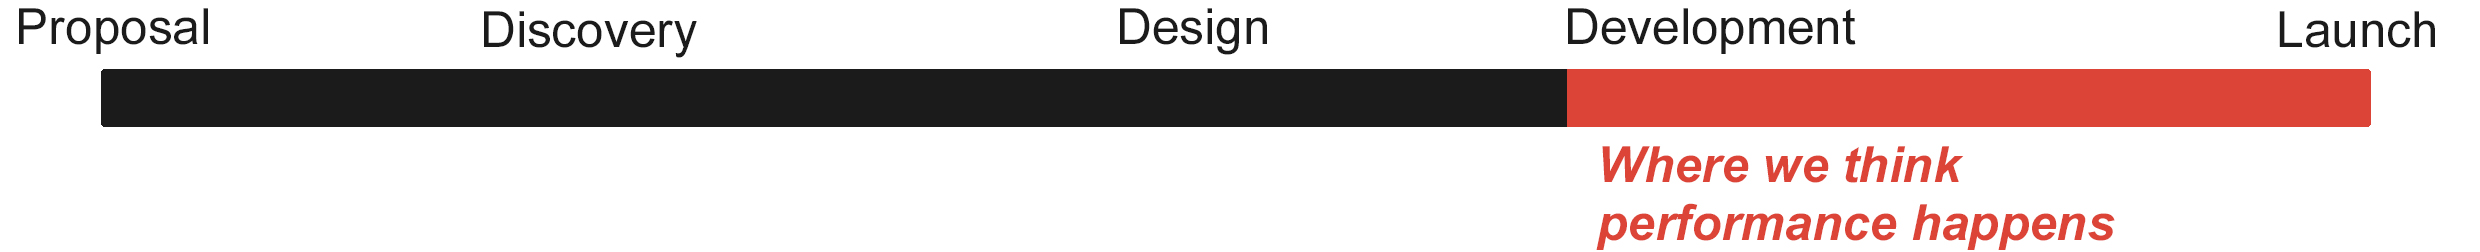
\includegraphics[width=\textwidth]{where_we_think_perf_happens.jpg}
			\caption{(Eigene Abbildung nach \autocite[p. 10]{kovalcin15})}
			\label{fig:where_we_think_perf_happens}
		\end{center}
	\end{figure}

	Genau das Gegenteil ist allerdings der Fall. Wenn eine Webanwendung klassischerweise in die Entwicklungsphase geht, sind bereits die meisten Weichen gestellt. Das Design ist ausgearbeitet und kann mehr oder weniger Mächtig ausfallen. Das Budget für das Projekt wurde vereinbart und der Umfang wurde Vertraglich festgelegt. Das Projektmanagement muss darauf achten, dass die Wünsche und Erwartungen des Kunden erfüllt werden und die Entwicklung sich auf diesen Aspekt konzentriert.

	\begin{figure}[htbp]
		\begin{center}
			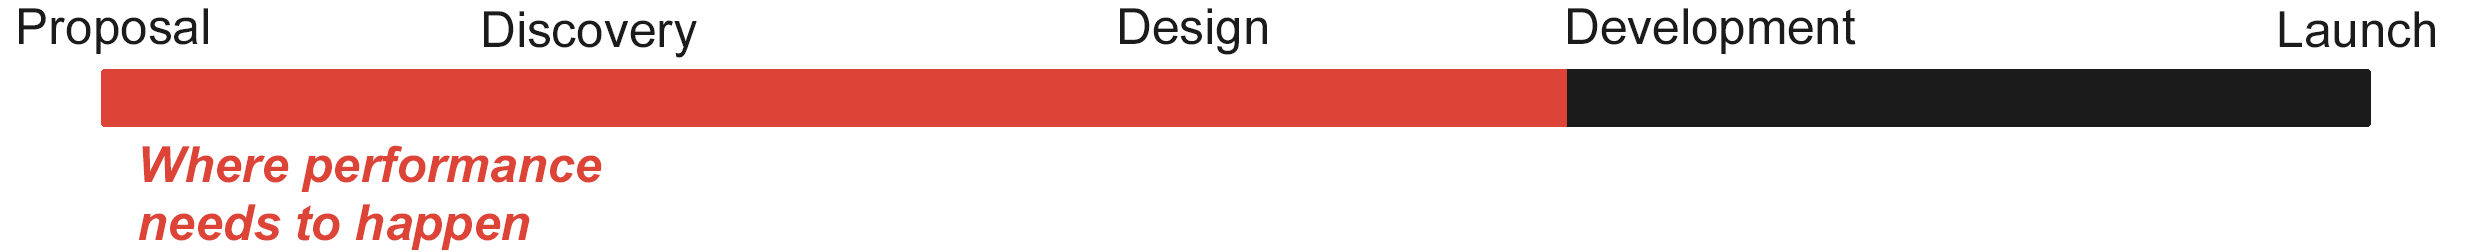
\includegraphics[width=\textwidth]{where_it_needs_to_happen.jpg}
			\caption{(Eigene Abbildung nach \autocite[p. 11]{kovalcin15})}
			\label{fig:where_it_needs_to_happen}
		\end{center}
	\end{figure}

	Deshalb beginnt das Thema Web Performance schon bereits ganz am Anfang. Der Kunde muss mit in das Boot geholt werden und es muss verdeutlicht werden, warum sich schnelle Ladezeiten lohnen, was für negative Auswirkungen langsame und was für positive Auswirkungen schnelle Ladezeiten auf den Endanwender haben. Der Kunde sieht oftmals nicht den Mehrwert an einer schnellen Webanwendung und möchte für etwas, dass er nicht sehen kann auch kein Geld investieren. Argumente wie:
	\begin{quote}
		\textit{"`We surveyed 3000 users about 17 key product drivers. They rated speed 2nd most important only after easy to find content."'} \autocite[p. 8]{hamann14}

		\textit{"`User load time expectations are 2 seconds or less and decreasing"'} \autocite{bixby13}
	\end{quote}
	oder die in dieser Arbeit genannten Argumente können bei der Überzeugungsarbeit helfen.\footnote{Eine Sammlung mit Argumenten ist im Anhang unter Punkt \ref{sub:argumentations_sammlung} zu finden.} Aktuelle Reports oder Zahlen und Fakten die den direkten Zusammenhang zwischen Ladezeit und dem daraus resultierenden Profit verdeutlichen sind, entsprechend aufbereitet, sehr hilfreich.\\
	Der Kunde könnte auch Argumentieren, dass er gar nicht so viele Mobile Anwender hat und es sich deshalb nicht lohnt. Dies war damals die selbe Argumentationsweise, die gegen "`Responsive Webdesign"' sprach. \textit{"`Amongst the top 10,000 websites, almost 8\% of websites went responsive within the span of a single year – an incredible growth!"'}\autocite{guypo14}. Diese Argumentation hielt nicht lange und heute spricht jede Firma von Responsive, will eine Responsive Website oder hat zumindest darüber nachgedacht.\autocite{guypo14} Web Performance ist ein Zukunftstrend, der mit der steigenden Anzahl an Smartphone Nutzer einher geht und damit früher oder später für jeden relevant ist. Ein guter "`sales pitch"' könnte sein:
	\begin{quote}
		 \textit{"`We'll provide you with a \textbf{fast}, responsive, immersive online experience."'}\autocite[p. 32]{kovalcin15}
	\end{quote}
	Dem Kunden muss Performance als visuell greifbares Erlebnis präsentiert werden. Dabei sind nicht nur Diagramme sondern auch Tools wie Webpagetest sehr nützlich. Damit können Vergleichsvideos erstellt werden. Denkbar wäre zum Beispiel ein direkter Vergleich mit den Konkurrenzseiten zu zeigen. Auch ein Vorher- / Nachervergleich eines erfolgreichen Projekts könnte dem Kunden präsentiert werden. Zum Launch kann dann ein Vergleich mit pre- und post-Performance aufgezeigt werden.\\

		\subsubsection{Projekt Manager} % (fold)
		\label{ssub:projekt_manager}
			Für das Team der Projekt Manager ergeben sich laut Katie Kovalcin folgende Hürde: \autocite[p. 43]{kovalcin15}\\
			\begin{itemize}
				\item Understand the importance
				\item Advocate with clients
				\item Help maintain performance budget.
			\end{itemize}
			Zuerst müssen die Projekt Manager verstehen, warum Web Performance wichtig für das Projekt ist um den Kunden entsprechend führen und beraten zu können. Des weiteren muss jemand dafür Sorge tragen, dass das Performance Budget (dazu später mehr) eingehalten wird. Neue Anforderungen und features müssen dementsprechend bewertet und mit dem Kunden diskutiert werden.\\
		% subsubsection projekt_manager (end)

		\subsubsection{Aesthetic heavy designers} % (fold)
		\label{ssub:aesthetic_heavy_designers}
			"`Aesthetic heavy designers"' können oft nicht abschätzen, was ihre Entscheidungen für einen Einfluss auf die Webanwendung haben. Die voraussetzung dafür ist zu wissen, wie das Web funktioniert. Warum Webanwendungen langsam sind und was dazu führt. Erst dann lassen sich Entscheidungen treffen, die sowohl den Endanwender und sein Online Erlebnis, als auch den ästhetischen Anspruch zufriedenstellen.	Wikipedia beschreibt den Begriff Design so:

			\begin{quote}
				\textit{"`Insbesondere umfasst Design auch die Auseinandersetzung des Designers \textbf{mit der Funktion eines Objekts sowie mit dessen Interaktion mit einem Benutzer}"'} \autocite{wikipediaDesign}
			\end{quote}

			Design ist also mehr als nur die visuelle Aufbereitung von Informationen, es muss in erster Linie dem Anwender dienen. Webseiten die zu groß sind, zerstören den Ansatz von Web Performance bereits schon zu Beginn. Wie in Punkt \ref{sub:perceived_performance} gesagt, verlassen über 50\% der Nutzer eine Seite nach einer Verzögerung von nur 3 Sekunden. Die emotionsvollsten Bilder und das prächtigste Design kann dem Besucher keine Botschaft vermitteln, wenn sie niemals zu sehen sein werden.

			\begin{quote}
				\textit{"`When you want to be fast, you have to \textbf{give up} the things slowing you down."'}\autocite[p. 2]{osmani14}
			\end{quote}

			Performance darf nicht als schlimmster Feind, sondern muss als bester Freund betrachtet werden. Dabei findet ein Balanceakt statt. Manchmal werden Entscheidungen zugunsten der Performance, ein anderes mal für die Ästhetik getroffen. Der Schlüssel ist es, alle verfügbaren Informationen zu nutzen, um die richtigen Entscheidungen für sich und die Webanwendung zu treffen.\autocite[p. 126]{laraHogan14}\\
			Der Designer muss sich Fragen stellen wie: "`Welchen Mehrwert hat der Nutzer durch dieses große Bild auf der Startseite"', braucht es 3 Schriftarten um einen gewissen \texttt{Look \& Feel} zu vermitteln oder reicht eine? Gibt es eine alternative Schriftart die fast identisch aussehen, aber viel weniger Bytes benötigt? 

			\begin{longtable}{|>{\raggedright \arraybackslash}p{4.9cm}|>{\raggedright \arraybackslash}p{4.9cm}|>{\raggedright \arraybackslash}p{5cm}|}
			\caption{Beispiel: Abwägung - Performance oder Ästhetik  (Tabelle nach \autocite[p. 126]{laraHogan14})}\\
			\hline
				\textbf{Question} & \textbf{Aesthetische Consideration} & \textbf{Performance Consideration}\\
				\hline
				Can I put a large hero image at the top of every page? & Eye-catching represents the brand & This could be a really large file, we want to minimize page weight\\
				\hline
				Should I use three Font-Weights plus a text weight? & Lots of flexibility in typography & We want to reduce page weight and requests\\
				\hline
				Do I need a carousel on the landing page? & Showcases lots of different content & This adds a lot of page weight and additional requests. The user might never see the 2nd image.\\
				\hline
				How can I demonstrate the product functionalities? & Could use a GIF or embed a video & Videos and GIF's can be very heavy.\\
				\hline
			\end{longtable}

			Die Antworten können je nach Projekt oder Designer unterschiedlich ausfallen.

			\begin{longtable}{|>{\raggedright \arraybackslash}p{7.6cm}|>{\raggedright \arraybackslash}p{7.6cm}|}
			\caption{Beispiel: Entscheidungen (Tabelle nach \autocite[p. 127]{laraHogan14})}\\
				\hline
				\textbf{Question} & \textbf{Decision}\\
				\hline
				Can I put a large hero image at the top of very page? & Yes, we use responsive images for the different screen sizes and compress them to reduce page weight! We might lose image quality.\\
				\hline
				Should I use three Font-Weights plus a text weight? & We need the 3 Font-Weights, they are used by the brand. No choice there\\
				\hline
				Do I need a carousel on the landing page? & No the extra images are not increasing the users experience.\\
				\hline
				How can I demonstrate the product functionalities? & We will use CSS-Animations instead of a GIF. This will cost some of the developers time.\\
				\hline	
			\end{longtable}

			Für viele Entscheidungsschritte macht es oft Sinn, dass Entwickler und Designer kollaborieren. Dabei können bereits zu einem sehr frühen Zeitpunkt \texttt{Bottlenecks} erkannt, alterantiven vorgeschlagen und diskutiert werden. Dafür muss es klare Regeln geben. So haben Phrasen wie: "`Das ist zu schwierig, gefällt mir nicht, dumme Idee, da gibt es keine Alternative, das Bild muss genau so aussehen"' generell nichts verloren. Viel mehr Sinn macht es Alternativen zu erarbeiten, Prioritäten zu diskutieren oder Lösungen aufzuzeigen. Ebeneso kann es hilfreich sein, früh mit einem Mockup oder Prototyp auf Code-Basis anzufangen und gemeinsam an diesem Dinge auszuprobieren.

			\begin{figure}[htbp]
				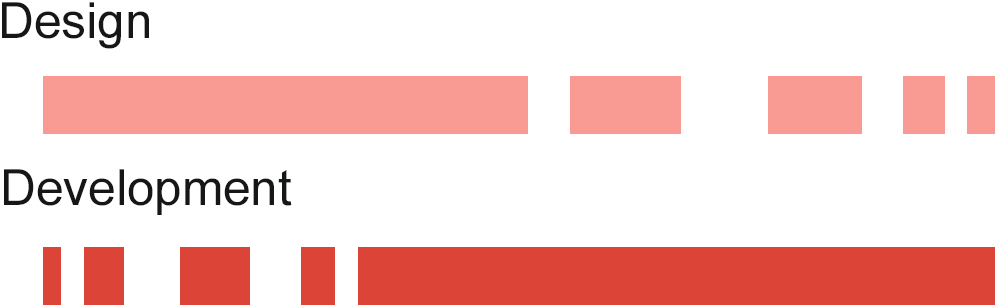
\includegraphics[width=0.5\textwidth]{project_timeline.jpg}
				\caption{Projekt Zeitlinie}
				\label{fig:project_timeline}
			\end{figure}
			
			Auch hier gilt wieder den Balanceakt zwischen Ästhetik und Performance zu finden und nicht gegeneinander sondern miteinander zu arbeiten. Um dem ganzen einen Rahmen zu geben, in dem sich sowohl Designer, Entwickler als auch der Kunde bewegen darf, wird von vielen Performance Führsprechern ein sogenanntes "`Performance Budget"' verwendet.
		
		% subsubsection aesthetic_heavy_designers (end)

		\subsubsection{Performance Budget} % (fold)
		\label{ssub:performance_budget}

		

		- was ist ein performance budget?\\
		- welchen vorteil hat das arbeiten damit?\\
		- welche metriken gibt es?\\
		- wie bestimme ich das richtige Budget für das Projekt? -> how fast is fast enough -> how fast is my competitor and how mutch I have to be faster, so the user notices it?\\
		- arbeiten mit einem budget -> design -> developer -> kunde\\
		- Vorteil / Nachteil?\\


		% subsubsection performance_budget (end)

	% subsection hürden (end)

% section der_weg_zur_performance (end)

\pagebreak
